\documentclass[11pt]{article}
\usepackage{physics}
% NOTE: Add in the relevant information to the commands below; or, if you'll be using the same information frequently, add these commands at the top of paolo-pset.tex file. 
\newcommand{\name}{TA: Hossein Mohammadi}
\newcommand{\email}{hossein.mohammadi.00427@gmail.com}
\newcommand{\classnum}{Advanced Quantum Field Theory}
\newcommand{\subject}{Subject: Path Integrals}
\newcommand{\instructors}{Dr. Amin Faraji}
\newcommand{\assignment}{PSet 2}
\newcommand{\semester}{- Fall 1402}
\newcommand{\duedate}{dd/mm/yyyy}
% Copyright 2021 Paolo Adajar (padajar.com, paoloadajar@mit.edu)
% 
% Permission is hereby granted, free of charge, to any person obtaining a copy of this software and associated documentation files (the "Software"), to deal in the Software without restriction, including without limitation the rights to use, copy, modify, merge, publish, distribute, sublicense, and/or sell copies of the Software, and to permit persons to whom the Software is furnished to do so, subject to the following conditions:
%
% The above copyright notice and this permission notice shall be included in all copies or substantial portions of the Software.
% 
% THE SOFTWARE IS PROVIDED "AS IS", WITHOUT WARRANTY OF ANY KIND, EXPRESS OR IMPLIED, INCLUDING BUT NOT LIMITED TO THE WARRANTIES OF MERCHANTABILITY, FITNESS FOR A PARTICULAR PURPOSE AND NONINFRINGEMENT. IN NO EVENT SHALL THE AUTHORS OR COPYRIGHT HOLDERS BE LIABLE FOR ANY CLAIM, DAMAGES OR OTHER LIABILITY, WHETHER IN AN ACTION OF CONTRACT, TORT OR OTHERWISE, ARISING FROM, OUT OF OR IN CONNECTION WITH THE SOFTWARE OR THE USE OR OTHER DEALINGS IN THE SOFTWARE.

\usepackage{fullpage}
\usepackage{enumitem}
\usepackage{amsfonts, amssymb, amsmath,amsthm}
\usepackage{mathtools}
\usepackage[pdftex, pdfauthor={\name}, pdftitle={\classnum~\assignment}]{hyperref}
\usepackage[dvipsnames]{xcolor}
\usepackage{bbm}
\usepackage{graphicx}
\usepackage{mathrsfs}
\usepackage{pdfpages}
\usepackage{tabularx}
\usepackage{pdflscape}
\usepackage{makecell}
\usepackage{booktabs}
\usepackage{natbib}
\usepackage{caption}
\usepackage{subcaption}
\usepackage{physics}
\usepackage[many]{tcolorbox}
\usepackage{version}
\usepackage{ifthen}
\usepackage{cancel}
\usepackage{listings}
\usepackage{courier}

\usepackage{tikz}
\usepackage{istgame}
\usepackage{Float}

\hypersetup{
	colorlinks=true,
	linkcolor=blue,
	filecolor=magenta,
	urlcolor=blue,
}

\setlength{\parindent}{0mm}
\setlength{\parskip}{2mm}

\setlist[enumerate]{label=({\alph*})}
\setlist[enumerate, 2]{label=({\roman*})}

\allowdisplaybreaks[1]

\newcommand{\psetheader}{
	\ifthenelse{\isundefined{\collaborators}}{
		\begin{center}
			{\setlength{\parindent}{0cm} \setlength{\parskip}{0mm}
				
				\textbf{\classnum~\semester:~\assignment} \hfill \name
				
				
				\subject \hfill %\href{mailto:\email}{\tt \email}
				
				Instructor:~\instructors \hfill Due Date:~\duedate	
				
				\hrulefill}
		\end{center}
	}{
		\begin{center}
			{\setlength{\parindent}{0cm} \setlength{\parskip}{0mm}
				
				{\textbf{\classnum~\semester:~\assignment} \hfill \name\footnote{Collaborator(s): \collaborators}}
				
				\subject \hfill \href{mailto:\email}{\tt \email}
				
				Instructor(s):~\instructors \hfill Due Date:~\duedate	
				
				\hrulefill}
		\end{center}
	}
}

\renewcommand{\thepage}{\classnum~\assignment \hfill \arabic{page}}

\makeatletter
\def\points{\@ifnextchar[{\@with}{\@without}}
\def\@with[#1]#2{{\ifthenelse{\equal{#2}{1}}{{[1 point, #1]}}{{[#2 points, #1]}}}}
\def\@without#1{\ifthenelse{\equal{#1}{1}}{{[1 point]}}{{[#1 points]}}}
\makeatother

\newtheoremstyle{theorem-custom}%
{}{}%
{}{}%
{\itshape}{.}%
{ }%
{\thmname{#1}\thmnumber{ #2}\thmnote{ (#3)}}

\theoremstyle{theorem-custom}

\newtheorem{theorem}{Theorem}
\newtheorem{lemma}[theorem]{Lemma}
\newtheorem{example}[theorem]{Example}

\newenvironment{problem}[1]{\color{black} #1}{}

\newenvironment{solution}{%
	\leavevmode\begin{tcolorbox}[breakable, colback=green!5!white,colframe=green!75!black, enhanced jigsaw] \proof[\scshape Solution:] \setlength{\parskip}{2mm}%
	}{\renewcommand{\qedsymbol}{$\blacksquare$} \endproof \end{tcolorbox}}

\newenvironment{reflection}{\begin{tcolorbox}[breakable, colback=black!8!white,colframe=black!60!white, enhanced jigsaw, parbox = false]\textsc{Reflections:}}{\end{tcolorbox}}

\newcommand{\qedh}{\renewcommand{\qedsymbol}{$\blacksquare$}\qedhere}

\definecolor{mygreen}{rgb}{0,0.6,0}
\definecolor{mygray}{rgb}{0.5,0.5,0.5}
\definecolor{mymauve}{rgb}{0.58,0,0.82}

% from https://github.com/satejsoman/stata-lstlisting
% language definition
\lstdefinelanguage{Stata}{
	% System commands
	morekeywords=[1]{regress, reg, summarize, sum, display, di, generate, gen, bysort, use, import, delimited, predict, quietly, probit, margins, test},
	% Reserved words
	morekeywords=[2]{aggregate, array, boolean, break, byte, case, catch, class, colvector, complex, const, continue, default, delegate, delete, do, double, else, eltypedef, end, enum, explicit, export, external, float, for, friend, function, global, goto, if, inline, int, local, long, mata, matrix, namespace, new, numeric, NULL, operator, orgtypedef, pointer, polymorphic, pragma, private, protected, public, quad, real, return, rowvector, scalar, short, signed, static, strL, string, struct, super, switch, template, this, throw, transmorphic, try, typedef, typename, union, unsigned, using, vector, version, virtual, void, volatile, while,},
	% Keywords
	morekeywords=[3]{forvalues, foreach, set},
	% Date and time functions
	morekeywords=[4]{bofd, Cdhms, Chms, Clock, clock, Cmdyhms, Cofc, cofC, Cofd, cofd, daily, date, day, dhms, dofb, dofC, dofc, dofh, dofm, dofq, dofw, dofy, dow, doy, halfyear, halfyearly, hh, hhC, hms, hofd, hours, mdy, mdyhms, minutes, mm, mmC, mofd, month, monthly, msofhours, msofminutes, msofseconds, qofd, quarter, quarterly, seconds, ss, ssC, tC, tc, td, th, tm, tq, tw, week, weekly, wofd, year, yearly, yh, ym, yofd, yq, yw,},
	% Mathematical functions
	morekeywords=[5]{abs, ceil, cloglog, comb, digamma, exp, expm1, floor, int, invcloglog, invlogit, ln, ln1m, ln, ln1p, ln, lnfactorial, lngamma, log, log10, log1m, log1p, logit, max, min, mod, reldif, round, sign, sqrt, sum, trigamma, trunc,},
	% Matrix functions
	morekeywords=[6]{cholesky, coleqnumb, colnfreeparms, colnumb, colsof, corr, det, diag, diag0cnt, el, get, hadamard, I, inv, invsym, issymmetric, J, matmissing, matuniform, mreldif, nullmat, roweqnumb, rownfreeparms, rownumb, rowsof, sweep, trace, vec, vecdiag, },
	% Programming functions
	morekeywords=[7]{autocode, byteorder, c, _caller, chop, abs, clip, cond, e, fileexists, fileread, filereaderror, filewrite, float, fmtwidth, has_eprop, inlist, inrange, irecode, matrix, maxbyte, maxdouble, maxfloat, maxint, maxlong, mi, minbyte, mindouble, minfloat, minint, minlong, missing, r, recode, replay, return, s, scalar, smallestdouble,},
	% Random-number functions
	morekeywords=[8]{rbeta, rbinomial, rcauchy, rchi2, rexponential, rgamma, rhypergeometric, rigaussian, rlaplace, rlogistic, rnbinomial, rnormal, rpoisson, rt, runiform, runiformint, rweibull, rweibullph,},
	% Selecting time-span functions
	morekeywords=[9]{tin, twithin,},
	% Statistical functions
	morekeywords=[10]{betaden, binomial, binomialp, binomialtail, binormal, cauchy, cauchyden, cauchytail, chi2, chi2den, chi2tail, dgammapda, dgammapdada, dgammapdadx, dgammapdx, dgammapdxdx, dunnettprob, exponential, exponentialden, exponentialtail, F, Fden, Ftail, gammaden, gammap, gammaptail, hypergeometric, hypergeometricp, ibeta, ibetatail, igaussian, igaussianden, igaussiantail, invbinomial, invbinomialtail, invcauchy, invcauchytail, invchi2, invchi2tail, invdunnettprob, invexponential, invexponentialtail, invF, invFtail, invgammap, invgammaptail, invibeta, invibetatail, invigaussian, invigaussiantail, invlaplace, invlaplacetail, invlogistic, invlogistictail, invnbinomial, invnbinomialtail, invnchi2, invnF, invnFtail, invnibeta, invnormal, invnt, invnttail, invpoisson, invpoissontail, invt, invttail, invtukeyprob, invweibull, invweibullph, invweibullphtail, invweibulltail, laplace, laplaceden, laplacetail, lncauchyden, lnigammaden, lnigaussianden, lniwishartden, lnlaplaceden, lnmvnormalden, lnnormal, lnnormalden, lnwishartden, logistic, logisticden, logistictail, nbetaden, nbinomial, nbinomialp, nbinomialtail, nchi2, nchi2den, nchi2tail, nF, nFden, nFtail, nibeta, normal, normalden, npnchi2, npnF, npnt, nt, ntden, nttail, poisson, poissonp, poissontail, t, tden, ttail, tukeyprob, weibull, weibullden, weibullph, weibullphden, weibullphtail, weibulltail,},
	% String functions 
	morekeywords=[11]{abbrev, char, collatorlocale, collatorversion, indexnot, plural, plural, real, regexm, regexr, regexs, soundex, soundex_nara, strcat, strdup, string, strofreal, string, strofreal, stritrim, strlen, strlower, strltrim, strmatch, strofreal, strofreal, strpos, strproper, strreverse, strrpos, strrtrim, strtoname, strtrim, strupper, subinstr, subinword, substr, tobytes, uchar, udstrlen, udsubstr, uisdigit, uisletter, ustrcompare, ustrcompareex, ustrfix, ustrfrom, ustrinvalidcnt, ustrleft, ustrlen, ustrlower, ustrltrim, ustrnormalize, ustrpos, ustrregexm, ustrregexra, ustrregexrf, ustrregexs, ustrreverse, ustrright, ustrrpos, ustrrtrim, ustrsortkey, ustrsortkeyex, ustrtitle, ustrto, ustrtohex, ustrtoname, ustrtrim, ustrunescape, ustrupper, ustrword, ustrwordcount, usubinstr, usubstr, word, wordbreaklocale, worcount,},
	% Trig functions
	morekeywords=[12]{acos, acosh, asin, asinh, atan, atanh, cos, cosh, sin, sinh, tan, tanh,},
	morecomment=[l]{//},
	% morecomment=[l]{*},  // `*` maybe used as multiply operator. So use `//` as line comment.
	morecomment=[s]{/*}{*/},
	% The following is used by macros, like `lags'.
	morestring=[b]{`}{'},
	% morestring=[d]{'},
	morestring=[b]",
	morestring=[d]",
	% morestring=[d]{\\`},
	% morestring=[b]{'},
	sensitive=true,
}

\lstset{ 
	backgroundcolor=\color{white},   % choose the background color; you must add \usepackage{color} or \usepackage{xcolor}; should come as last argument
	basicstyle=\footnotesize\ttfamily,        % the size of the fonts that are used for the code
	breakatwhitespace=false,         % sets if automatic breaks should only happen at whitespace
	breaklines=true,                 % sets automatic line breaking
	captionpos=b,                    % sets the caption-position to bottom
	commentstyle=\color{mygreen},    % comment style
	deletekeywords={...},            % if you want to delete keywords from the given language
	escapeinside={\%*}{*)},          % if you want to add LaTeX within your code
	extendedchars=true,              % lets you use non-ASCII characters; for 8-bits encodings only, does not work with UTF-8
	firstnumber=0,                % start line enumeration with line 1000
	frame=single,	                   % adds a frame around the code
	keepspaces=true,                 % keeps spaces in text, useful for keeping indentation of code (possibly needs columns=flexible)
	keywordstyle=\color{blue},       % keyword style
	language=Octave,                 % the language of the code
	morekeywords={*,...},            % if you want to add more keywords to the set
	numbers=left,                    % where to put the line-numbers; possible values are (none, left, right)
	numbersep=5pt,                   % how far the line-numbers are from the code
	numberstyle=\tiny\color{mygray}, % the style that is used for the line-numbers
	rulecolor=\color{black},         % if not set, the frame-color may be changed on line-breaks within not-black text (e.g. comments (green here))
	showspaces=false,                % show spaces everywhere adding particular underscores; it overrides 'showstringspaces'
	showstringspaces=false,          % underline spaces within strings only
	showtabs=false,                  % show tabs within strings adding particular underscores
	stepnumber=2,                    % the step between two line-numbers. If it's 1, each line will be numbered
	stringstyle=\color{mymauve},     % string literal style
	tabsize=2,	                   % sets default tabsize to 2 spaces
%	title=\lstname,                   % show the filename of files included with \lstinputlisting; also try caption instead of title
	xleftmargin=0.25cm
}


% NOTE: To compile a version of this pset without problems, solutions, or reflections, uncomment the relevant line below.

%\excludeversion{problem}
%\excludeversion{solution}
%\excludeversion{reflection}

\begin{document}	
	
	% Use the \psetheader command at the beginning of a pset. 
	\psetheader
	
	\section*{Problem 1: Grassmannian Path Integrals }
	
	\begin{problem}
		In this problem, we will review some essential concepts regarding non-commutative path integrals.
	\end{problem}
	\begin{enumerate}
		\item
		\begin{problem}{\points[9.5 Peskin]{-}}
			\textbf{Basic properties of Grassmann numbers:}
			
			\noindent
			The basic fact about these numbers is that they anti-commute, $\eta\theta = -\theta \eta$. Hence they square to zero, $\theta^2 = 0$.‌ Argue that any function of Grassmann number is a linear function, $f(\eta) = A\eta+B$.
			
			\noindent
			\textbf{Aside:} In light of $\theta^2=0$, can we conclude that terms such as $\bar{\psi} \psi \bar{\psi} \psi$ or $(\bar{\psi}\psi)^2$ vanish in Lagrangian? As an instance, 4-Fermi theory has the former term.
		\end{problem}
		\item
		\begin{problem}{\points[9.5 Peskin]{-}}
		\textbf{Integration of Grassmann valued functions:}
		
		We define $\int d\theta (A+B\theta) = B$. Justify this definition by considering a change of variable $\theta \xrightarrow{} \theta + \eta$.
		\end{problem}
	\item
	\begin{problem}{\points[9.5 Peskin]{-}}
		\textbf{A simple Integration:}
		
		\noindent
		Let's play more with this interesting variables.

		\begin{enumerate}
			\item To warm up, compute $\int d\bar{\theta}d\theta e^{-\bar{\theta}b\theta}$, where $b$ is an ordinary number.[ Just expand this integral and use the $\theta^2= \bar{\theta}^2 =0$ property.]
			\item Compute $\int d\bar{\theta}d\theta\;\bar{\theta}\theta e^{-\bar{\theta}b\theta}$, where $b$ is an ordinary number.[ Notice the importance of ordering of Grassmann variables, unless we will have a minus ambiguity.]
			\item To generalize to multi-variable case, consider the following integral:
			\[
			\int d\bar{\theta}_1 \dots  d\bar{\theta}_n d\theta_1 \dots d\theta_n e^{-\bar{\theta}_i A_{ij} \theta_j}
			\]
			Where $A_{ij}$ is a $n\times n$ matrix. Work out this formula. [Expand the exponential and decide which terms survive. You must end up to $\det(A)$.]
			\item $[\text{Optional}]$ Another way of doing this, as Peskin does, is utilizing defintion of Jacobian of transformation in the Grassmann variables. This is a simple exercise that could be accompllished.

			
		\end{enumerate}
	\end{problem}
\end{enumerate}



\newpage

\section*{Problem 2: Path Integral Manual Dexterity}
\begin{problem}
	In this problem, we use all our knowledge to quantize elementary theories by path integrals. 
	Scalar QED and establishing the equivalence of correlation functions in second-quantized and path integral quantizations, are subjects of this exercise.
\end{problem}	

	\begin{enumerate}
	\item
	\begin{problem}{\points[Peskin Problem 9.1]{-}}
		\textbf{Scalar QED:} 
		
		\noindent
		This problem concerns the scalar QED theory of a complex field $\phi$ interacting with the electromagnectic potential $A^\mu$. The lagrangian is 
		\[
		\mathscr{L} = -\frac14 F_{\mu\nu}^2 + (D_\mu \phi)^{*} (D^\mu\phi) - m^2\phi^{*}\phi
		\]
		Where $D_\mu = \partial_\mu + ieA_\mu$.
		
		\noindent
		Use the functional methods discussed in Section 9.2, show that the following are Feynmann rules of this theory.
		
		\begin{figure}[H]
			\centering
			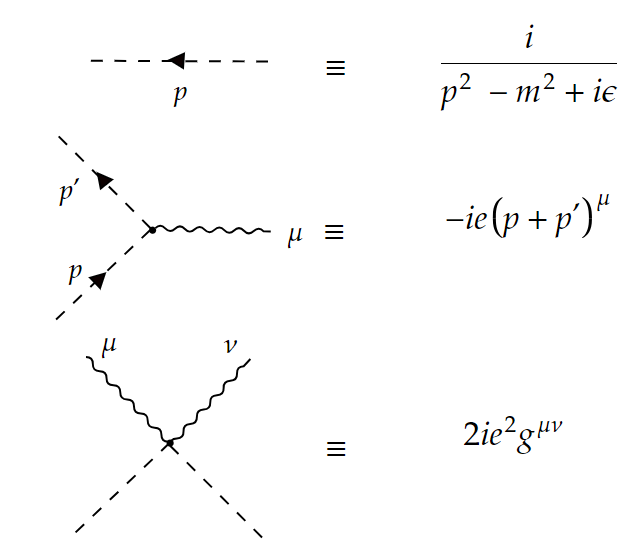
\includegraphics[width=0.5\linewidth]{img/1.png}
			\caption{Scalar QED basic Feynman diagrams.}
		\end{figure}
	\end{problem}
	\item
	\begin{problem}{\points{-}}
		\textbf{Correlation functions in different quantization schemes}
		
		\noindent
		 We want to establish the equivalence between n-point functions in second-quantization and path integal quantization.
		 
		\noindent
		\begin{enumerate}
			\item 
			Using what we've learned in the classroom about generating functionals and sources $J$, prove that second quantized n-point function 
			\[
			\bra{\Omega} T{\phi(x_1) \dots \phi(x_n)} \ket{\Omega} = \frac{
		\bra{0} T\{\phi_0(x_1) \dots \phi_0(x_n) e^{i\int d^4x \mathscr{L}_{int}[\phi]}\}\ket{0}	
		}{
\bra{0} T\{ e^{i\int d^4x \mathscr{L}_{int}[\phi]}\}\ket{0}		
}
			\],
			is equivalent to 
			\[
			(-i)^n \frac{1}{Z[0]} \frac{\partial^n Z}{\partial J(x_1) \dots \partial J(x_n)} \Big|_{J=0}
			\].
			In first relation $\phi_0(x)$ is the Heisenberg picture fields in free-theory and in the second, $Z[J]$ is generating functional of the full theory.
			
			\noindent
			[Despite its formidable appearance, it's a trivial question. Don't be afraid and start by divding full Lagrangian into $\mathscr{L} = \mathscr{L}_{free} + \mathscr{L}_{int}$, then plug it into path integral and use the relation between path-integral and n-point function in "Free Theories".]
			
			\item  Now that you've proved the most general case, let's verify it for $\phi^3$ theory, where $\mathscr{L}_{int} = \frac{g}{3!} \phi^3$. Expand $e^{i\int d^4 \mathscr{L}_{int}}$ in the path integral and conclude that two point function in this interactive theory gives the same result as Feynman rules up to order $g^4$.
		\end{enumerate}
	\end{problem}





\end{enumerate}


\newpage
\section*{Problem 3: Quantum Statistical Mechanics}
\begin{problem}
	We work out the world's most famous problem in the path integral formalism. These problems are 9.2 (a) and (b), Peskin.
\end{problem}	

\begin{enumerate}
	\item
	\begin{problem}{\points[Peskin Problem 9.2 (a)]{-}}
		\textbf{Quantum Statistical Mechanics} 
		
		\noindent
		Solve problem 9.2 (a), which is a review of quantum mechanical path integral, but in Euclidean signature.
	\end{problem}
	\item
	\begin{problem}{\points[Peskin Problem 9.2 (b)]{-}}
		\textbf{Harmonic Oscillator Path Integral}
		
		\noindent
	Now work out the part (b). Use the fourier expansion suggested, plug into path integral. The integration is a bit baffling, but pay close attention to (9.23) to figure out how to do these integrals. You will eventally end up with an infinite product, which turns out to be $\sinh(z)$, as suggested in the question. This gives the correct partition function for quantum mechanical oscillators, one that you've read in advanced statistical mechanics courses.
	\end{problem}
	
	
	
	
	
\end{enumerate}






\noindent
\begin{reflection}
	There are many interesting ideas in path integrals:
	\begin{itemize}
		\item  Schwinger Dyson equations: this equations govern the expectation values of the field operators, and bear a close resemblance to classical counterparts up to contact terms.
		\item Noether current and other symmetries: this is surprising how a simple change of variables in path integral could give us Noether current and Ward-Takahashi identity in QED.
		\item Quantization of QED: this is also a general procedure to quantize spin-1 fields, discussed in your textbook, I hope you cover these parts too.
	\end{itemize}
\end{reflection}

\end{document}